% globale Parameter (Papierformat, Schriftgroeße, Trennlinien, Doppelseitig)
\documentclass[a4paper, 11pt, headsepline,footsepline,twoside,abstract]{scrbook}


%%% Verwendete Pakete %%%

\usepackage{url}
\usepackage{geometry} % Seitenraender
\usepackage{fancyhdr} % Schoenere Kopf/Fußzeilen
\usepackage[utf8]{inputenc} % Kodierung
\usepackage[ngerman]{babel} % Sprache
\usepackage{graphicx}  % Bildchen
\usepackage{float}  % Bildchen2
\usepackage{setspace} % fuer Zeilenabstand
\usepackage[T1]{fontenc} % fuer Schriftart
%\usepackage{cite} % fuer Zitate
\usepackage[numbers,square]{natbib} % Package für Zitierstil
\usepackage{pgfplots} % Plots
\usepackage[justification=RaggedRight, singlelinecheck=false, margin=1.5cm]{caption}  % huebschere Captions
\usepackage[version=3]{mhchem} % chemische Formeln
\usepackage{booktabs} % schoenere Tabellen
\usepackage{multirow} % s.o.
\usepackage{ifthen} % s.o.
\usepackage{subfigure} % Grafiken nebeneinander darstellen
\usepackage{textcomp} %Euro-Zeichen
\usepackage{siunitx} % Einheiten korrekt anzeigen
\sisetup{
  locale = DE ,
  per-mode = symbol,
  separate-uncertainty %+- Notation
}
\DeclareSIUnit{\masspercent}{m\%}
\newcommand{\euro}{\,\texteuro\ } %Euro einfuegen

%Schriftart aendern
\newcommand{\changefont}[3]{
\fontfamily{#1} \fontseries{#2} \fontshape{#3} \selectfont}
\changefont{ptm}{m}{n}

% Zeilenabstand 1,5
\onehalfspacing

% weniger breite Seitenraender
\geometry{a4paper,left=28mm,right=28mm, top=32mm, bottom=30mm} 

% Keine Einrueckung bei neuen Absätzen
%\setlength{\parindent}{0pt}
%\setlength{\parskip}{\baselineskip}

% Bissel Tabellenmagie
\newcommand{\forloop}[5][1]{%
\setcounter{#2}{#3}%
\ifthenelse{#4}{#5\addtocounter{#2}{#1}%
\forloop[#1]{#2}{\value{#2}}{#4}{#5}}%
{}}

\newcounter{crcounter}

\newcommand{\compensaterule}[1]{%
\forloop{crcounter}{1}{\value{crcounter} < #1}%
{\vspace*{-\aboverulesep}\vspace*{-\belowrulesep}}}

\newcommand{\multirowbt}[3]{\multirow{#1}{#2}%
{\compensaterule{#1}#3}}

%%% Kopf und Fußzeilendesigns %%%

% normaler Style
\fancypagestyle{normal}
{
\fancyhead[EL]{\thepage}
\fancyhead[ER]{\leftmark}
\fancyhead[OL] {\rightmark}
\fancyhead[OR]{\thepage}
\fancyfoot[OL]{\parbox[b][0.04\columnwidth][t]{0.5\textwidth}{\raggedright Seminararbeit, Christoph Gielisch}}
\fancyfoot[OR]{
	
\includegraphics[height=0.05\columnwidth]{images/KIT_LOGO.png}
	%\caption{}
	\label{img:grafik-dummy}
	}
\fancyfoot[OC,EC]{}
\fancyfoot[EL]{
	
\includegraphics[height=0.05\columnwidth]{images/KIT_LOGO.png}
	%\caption{}
	\label{img:grafik-dummy}
	}
\fancyfoot[ER]{\parbox[b][0.04\columnwidth][t]{0.5\textwidth}{\raggedleft  Evaluierung der Elektrodenstrukturierung für Batterien und Kondensatoren}}
\renewcommand{\headrulewidth}{0.5pt}
\renewcommand{\footrulewidth}{0.5pt}
}

% Kapitelanfaenge bekommen ein extra Kopf/Fußzeilendesign
\fancypagestyle{plain}
{
\fancyhf{} % clear all header and footer fields
\fancyfoot[R]{\parbox[b][0.04\columnwidth][t]{0.5\textwidth}{\raggedleft \thepage}}
\fancyfoot[L]{
	
\includegraphics[height=0.05\columnwidth]{images/leerpixel.png}
	%\caption{}
	\label{img:grafik-dummy}
	}
\renewcommand{\headrulewidth}{0pt}
\renewcommand{\footrulewidth}{0.5pt}
}

% Die Inhaltsangabe auch
\fancypagestyle{toc}
{
\fancyhf{} % clear all header and footer fields
\fancyfoot[OR]{\parbox[b][0.04\columnwidth][t]{0.5\textwidth}{\raggedleft \thepage}}
\fancyfoot[OL]{
	
\includegraphics[height=0.05\columnwidth]{images/leerpixel.png}
	%\caption{}
	\label{img:grafik-dummy}
	}
\fancyfoot[EL]{\parbox[b][0.04\columnwidth][t]{0.5\textwidth}{\raggedright \thepage}}
\fancyfoot[ER]{
	
\includegraphics[height=0.05\columnwidth]{images/leerpixel.png}
	%\caption{}
	\label{img:grafik-dummy}
	}
\renewcommand{\headrulewidth}{0pt}
\renewcommand{\footrulewidth}{0.5pt}
}

% Festlegung Art der Zitierung
%\bibliographystyle{unsrtdin}

%%%%%%%%%%%%%%%%%%% hier beginnt das Dokument %%%%%%%%%%%%%%%%%%%%
\begin{document}

\thispagestyle{empty}
\begin{center}
%\Large{Karlsruher Institut für Technologie}\\
\end{center}

\begin{figure}
	\centering
	
\includegraphics[width=0.5\columnwidth]{images/KIT_LOGO.png}
	%\caption{}
	\label{img:grafik-dummy}
\end{figure}

\begin{center}
\textbf{\huge{ Aufbau einer in-situ Li$^7$-NMR\\[0.4cm]Batterietestzelle}}
\end{center}
\begin{center}
\large{}
\end{center}
\begin{center}
\textbf{\Large{}}
\end{center}
\begin{center}
\large{Von der Fakultät für Wirtschaftswissenschaften des \\ Karlsruher Instituts für Technologie genehmigte }
\end{center}
\begin{verbatim}

\end{verbatim}
\begin{center}
\textbf{\LARGE{Masterarbeit}}
\end{center}
\begin{center}
am
\end{center}
\begin{center}
\textbf{\Large{Institut für Angewandte Materialien - Keramische Werkstoffe und Technologien (IAM-KWT)}}
\end{center}
\begin{center}
von
\end{center}
\begin{center}
\Large{Christoph Gielisch}
\end{center}
\begin{verbatim}

\end{verbatim}
\begin{center}
15. August 2015
\end{center}
\begin{verbatim}

\end{verbatim}
\begin{center}
\textbf{Referent:} \\ Prof. Dr-Ing. Volker Schulze \\
\textbf{Koreferent:} \\ Prof. Dr. Michael J. Hoffmann\\
\textbf{Betreuer:} \\ Dr. Claudia Bucharsky \\ 
Dr.-Ing. Günter Schell \\
\end{center}
\newpage
\cleardoubleemptypage
% Eidesstattliche Erklärung
\setcounter{page}{1}
\pagenumbering{Roman}
\textbf{\Large{Eidesstattliche Erklärung}}
\\\\
Hiermit erkläre ich, diese Arbeit selbstständig und ohne fremde Hilfe verfasst zu haben. Es wurden nur die in der Arbeit ausdrücklich benannten Quellen und Hilfsmittel benutzt. Wörtlich oder sinngemäß übernommenes Gedankengut ist als solches gekennzeichnet.
\\\\
Karlsruhe, den 15.08.2015
\\\\
\\\\
\\
(Christoph Gielisch) 
 
\newpage

% Eidesstattliche Erklärung2
\setcounter{page}{1}
\pagenumbering{Roman}
\textbf{\Large{Zusammenfassung}}
\\\\
Es ist möglich die Oberfläche von Aluminiumfolien für den Einsatz als Stromkollektor in Batterien gezielt zu strukturieren. Es ist gelungen, strukturierte Folien zu funktionalen \ce{LiCoO2}-Elektroden zu verarbeiten und in Testzellen einzusetzen. Mit Hilfe einer Impedanzspektroskopie konnte der Widerstand zwischen Stromkollektor und Aktivmaterial untersucht werden. Dabei zeigte eine sandgestrahlte Aluminiumoberfläche ein verbessertes Verhalten gegenüber einer unbearbeiteten Oberfläche. Für einen wirtschaftlichen Einsatz der Technologie sind allerdings weitere Untersuchungen hinsichtlich der Fertigung mit Roll-to-Roll-Anlagen notwendig.
% Inhaltsverzeichnis
%\KOMAoption{open}{left} 
\pagestyle{toc}
\renewcommand*{\chapterpagestyle}{toc} % Die erste Seite des TOC ist auch ein Kapitelanfang
\tableofcontents
\KOMAoption{open}{right} 
\newpage
\cleardoubleemptypage
\pagestyle{normal}
\renewcommand*{\chapterpagestyle}{plain}
\setcounter{page}{1}
\pagenumbering{arabic}
\chapter{Einleitung}
Batterien und Kondensatoren sind bereits heutzutage in den meisten elektrischen Geräten verbaut. Im Rahmen des Klimaschutzes ist in Zukunft ein stärkerer Einsatz von elektrischen Komponenten als Substitut für bisher mittels fossiler Brennstoffe betriebener Geräte und Maschinen zu erwarten. In den letzten Jahren konnte die Leistungsfähigkeit von Batterien schon beträchtlich gesteigert werden, wie Abbildung 1.1 verdeutlicht. Im Rahmen dieser Arbeit soll die Möglichkeit einer weiteren Verbesserung durch Mikrostrukturierung der Elektroden sowie deren wirtschaftliche Machbarkeit überprüft werden.
\\
\begin{figure}[h]
\centering
\begin{tikzpicture}[thick, scale=1.0]
	\begin{axis}[
		% title =  \textbf{\large{Testtitel}},
		legend style = {draw=none},
		legend pos = outer north east,
		xlabel = Jahr,
		xmax = 2005,
		xmin = 1985,
		xtick={1985,1990,1995,2000,2005},
 		x tick label style={/pgf/number format/1000 sep=},
		ylabel = Energiedichte in Wh/kg,
		ymax = 200,
		ymin =0,
		ytick={50,100,150,200},
		scale only axis, % The height and width argument only apply to the actual axis
		height=6cm,
		width=\textwidth-\widthof{100}-5.0cm, % \textwidth minus width of longest label text minus label offset
		yticklabel style={align=right,inner sep=0pt,xshift=-0.1cm} % No inner sep, to remove whitespace on left, manually offset by given distance
		]

		\addplot[
			color = black,
			%fill = black,
			mark = *, % * = leer
			%only marks
			]
 		coordinates {
			( 1985, 25 )
			( 1991, 40 )
			( 1995, 45 )
			( 2000, 52 )
			( 2004, 63 )
			};

		\addlegendentry{NiCd}

		\addplot[
			color = blue,
			%fill = black,
			mark = *, % * = leer
			%only marks
			]
 		coordinates {
			( 1989, 50 )
			( 1993, 60 )
			( 1996, 75 )
			( 1999, 85 )
			( 2002, 95 )
			( 2004, 105)
			};

		\addlegendentry{NiMH}

		\addplot[
			color = red,
			%fill = black,
			mark = *, % * = leer
			%only marks
			]
 		coordinates {
			( 1994, 110 )
			( 1996, 130 )
			( 1998, 150 )
			( 2000, 165 )
			( 2004, 190 )
			};

		\addlegendentry{Li-Ionen}

	\end{axis}
\end{tikzpicture}
\caption{Entwicklung der Energiedichten verschiedener Batteriesysteme (\cite{jossen_2006}, S.129)}
\end{figure}
\\
\vspace{0.3cm}
\textbf{\large{Zielsetzung und Herangehensweise}}\\
%\section{Zielsetzung und Herangehensweise}
Im Folgenden werden zunächst die Grundlagen der eingesetzten Technologien erläutert. Es werden Kennzahlen definiert, die als Gradmesser für die Leistungsfähigkeit und Wirtschaftlichkeit einer möglichen Fertigung dienen. Anschließend werden das Verfahren, die dabei eingesetzten Maschinen und die gewonnen Ergebnisse vorgestellt. Die so ermittelte Datengrundlage wird dann in Kapitel \ref{discussion} weiter diskutiert. Dabei wird neben der Eignung der Strukturierung für Batterieanwendungen auch deren Wirtschaftlichkeit untersucht. Schlussendlich werden die gewonnenen Erkenntnisse zusammengefasst und ein Ausblick auf die Zukunft gegeben.
\newpage
\chapter{Grundlagen}
Für die spätere Optimierung der Strukturierung ist es nötig, die Funktionsweise von Batterien und Kondensatoren sowie die Prozessierung zu verstehen. Für die wirtschaftliche Einordnung wird ein kurzer Überblick über verschiedene Kennzahlen zur Valuierung gegeben.
\section{Funktionsweise von Batterien und Kondensatoren}
Batterien und Kondensatoren sind in der Lage elektrische Energie zu speichern, benutzen dafür allerdings unterschiedliche Mechanismen. Im Folgenden wird der Aufbau sowie die Funktionsweise beider kurz vorgestellt.
\subsection{Aufbau von Batterien}
\begin{figure}[b]
	\centering
	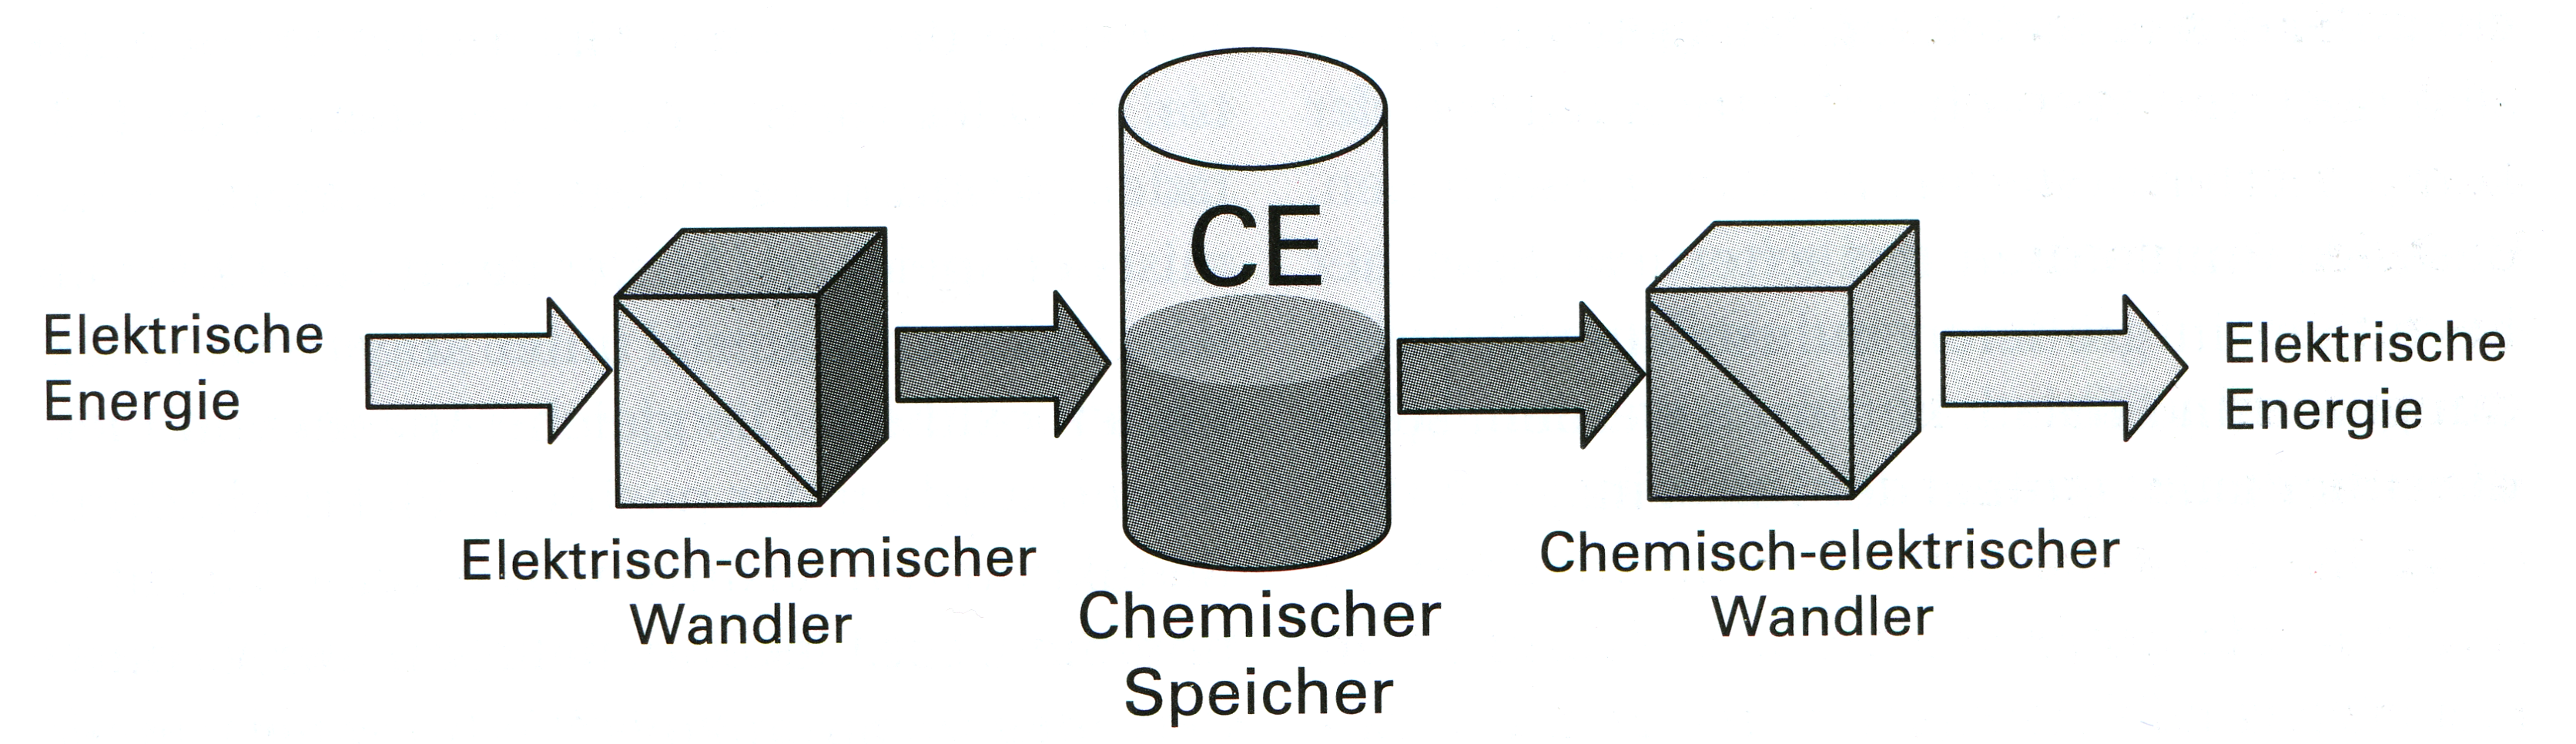
\includegraphics[width=1\columnwidth]{images/Prinzipieller_Aufbau.png}
	\caption{Prinzip der Energieumwandlung und Speicherung bei Batterien \cite{jossen_2006}.}
	\label{Prinzip Batterie}
\end{figure}
Eine Batterie ist aus elektrochemischen Zellen aufgebaut, die in der Lage sind, ihr chemisches Potential in Form von elektrischer Energie abzugeben. Je nach Typ unterscheidet Buchholz in \cite{buchholz2010} (S. 109) zwischen:
\begin{description}
\item[Primäre Zelle] Eine primäre Zelle ist in der Lage, das in ihr vorhandene chemische Potential in Form von elektrischer Energie abzugeben.
\item[Sekundäre Zelle] Im Deutschen häufig auch \textit{Akkumulator} genannt, im Englischen \textit{rechargeable battery}. Eine sekundäre Zelle besitzt neben der Eigenschaft eines Chemisch-elektischen-Wandlers auch die Rückfunktion, ist also auch ein Elektrisch-chemischer-Wandler und kann daher nicht nur chemisches Potential in elektrische Energie umwandeln, sondern auch elektrische Energie als chemisches Potential speichern.
\item[Tertiäre Zelle]  Bei einer Tertiären Zelle können von außen Reaktionsedukte zugeführt werden, die innerhalb der Zelle abreagieren und dabei einen elektrischen Strom produzieren. Anschließend werden diese als Produkte wieder abgeführt. Häufig wird diese Art von Zelle auch \textit{Brennstoffzelle} genannt.
\end{description}
Primäre Zellen sind nicht-wiederaufladbare Einmal-Batterien. Durch die fehlende Auflademöglichkeit sind die durch mehrmalige Ladevorgänge auftretenden Alterungsprozesse nicht vorhanden. In der Regel sind diese Batterien einfach und kostengünstig zu produzieren. Sie werden beispielsweise in Geräten mit geringem Energiebedarf eingesetzt, bei denen die Nutzungsdauer des Gesamtprodukts nur um wenige Faktoren über der Lebensdauer der Batterie liegt. Ein häufiger Vertreter dieser Gattung ist die Zink-Manganoxid-Zelle, die unter dem Namen Alkaline-Batterie bekannt ist. 
\\\\
Wiederaufladbare Batterien finden eine weite Verbreitung in vielen verschiedenen Einsatzfeldern. Waren zu Beginn des letzten Jahrhunderts noch vorwiegend Bleibatterien in Nutzung, so wurde nach dem Zweiten Weltkrieg die Nickel-Cadmium-Batterie immer beliebter, die ab Mitte der 90er von den Nickel-Metallhydrid-Batterien abgelöst wurde. In den letzten 15\;Jahren konnte mit der Entwicklung und kontinuierlichen Verbesserung der Lithium-Ionen-Batterie die Energie- und Leistungsdichte noch weiter gesteigert werden. Eine Übersicht aller Batterietechnologien ist in Abbildung \ref{uebersicht_technologien} zu sehen.
\begin{figure}[]
	\centering
	
\includegraphics[width=1\columnwidth]{images/Energiespeicher2.png}
	\caption{Energie- und Leistungsdichte verschiedener Batterietechnologien in der Übersicht \cite{wikimedia_energiespeicher}.}
	\label{uebersicht_technologien}
\end{figure}
\\\\
Im Rahmen dieser Arbeit werden lediglich Sekundäre Zellen betrachtet. Der Fokus liegt dabei auf Lithium-Ionen-Batterien. Eine Lithium-Ionen-Batteriezelle besteht dabei im Kern aus fünf Bauteilen (siehe \cite{korthauer2013}, S.14ff):
\begin{itemize}
\item \textbf{Anode:} Typische Anodenstoffe sind amorpher Kohlenstoff, Graphit, Lithiumoxide und -verbind\-ungen sowie Metalloxide. 
\item \textbf{Kathode:} Für die Kathode wird unter Anderem \ce{LiCoO2}, \ce{LiNiO2}, \ce{LiMn2O4} oder \ce{LiFePO4} eingesetzt. Zur besseren Haftung und Leitung werden Binder und Leitruße beigemengt.
\item \textbf{Elektrolyt:}  Der Elektrolyt ist eine Mischung aus einer wasserfreien Flüssigkomponente (ein Lösungmittel wie beispielsweise eine Ethylenkarbonat-Dimethylkarbonat-Mischung), einem lithiumhaltigen Leitsalz (\ce{LiPF6}, \ce{LiClO4}) und Zusätze wie Vinylidenkarbonat oder auch fein verteilte \ce{SiO2} oder \ce{Al2O3} Pulver.
\item \textbf{Seperator:}  Seperatoren bestehen aus hochporösen Plastikfolien aus Polyethylen oder Polypropylen. Diese wirken wie eine Membran, die durchlässig ist für die Ionen innerhalb des Elektrolyts, die Zelle aber vor dem inneren Kurzschluss bspw. durch Zusammenwachsen der Elektroden schützt.
\item \textbf{Stromkollektoren:} Die Stromkollektoren nehmen Elektronen vom Elektrodenmaterial auf oder geben sie an dieses ab. Dabei kann an sie ein Verbraucher angeschlossen werden, um so den Elektronenfluss als elektrischen Strom abzugreifen. In der Regel kommt dabei auf der Anodenseite Kupfer, auf der Kathodenseite Aluminium zum Einsatz.
\end{itemize}
Es existieren verschiedene Möglichkeiten zur Fertigung von Batteriezellen. Bei kleineren Batterien und in Testumgebungen kommen häufig \textit{Knopfzellen} zum Einsatz. Dabei werden die beiden Elektroden sowie auch die Kollektoren und Separatoren in Scheiben von mehreren Millimetern Durchmesser gestanzt und in einem flachen, kreisförmigen Metallgehäuse untergebracht. 
\\\\
Bei \textit{Rundzellen} sind die Stromkollektoren doppelseitig mit Elektrodenmaterial beschichtet. Die Batterie wird dann in Form eines Zylinders aufgewickelt. Auch die Wicklung mit einer rechteckigen Grundfläche ist möglich, dabei entsteht eine \textit{prismatische Zelle}. Beide Zellen werden anschließend in ein stabiles Gehäuse eingefasst. Dem gegenüber steht die in lediglich dünne Folie eingeschweißte \textit{Pouch-Zelle}. Eine Überischt über die verschiedenen Bauformen findet sich in der Abbildung \ref{vergleich_bauformen}.
\begin{figure}[h]
	\centering
	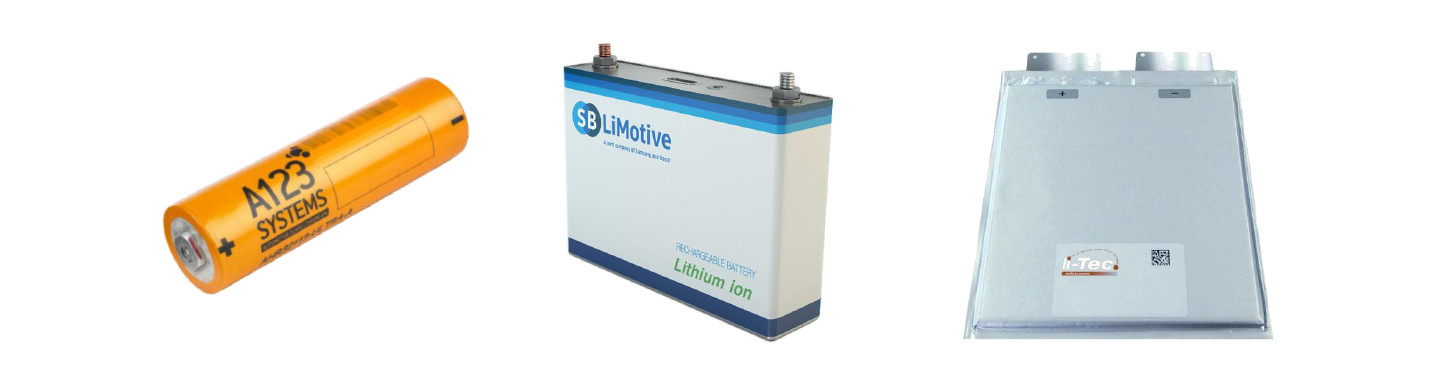
\includegraphics[width=1\columnwidth]{images/rund_prisma_pouch.jpg}
	\caption{Unterschiedliche Bauformen von Batterien (von links nach rechts): Rundzelle, prismatische Zelle, Pouch-Zelle \cite{bub_skript}.}
	\label{vergleich_bauformen}
\end{figure}
\\\\
Mehrere Batteriezellen können zu einem Batteriemodul zusammengeschlossen werden. Diese Module können weiterhin zu Battery-Packs kombiniert und durch ein zentrales Batteriemanagement gesteuert werden.
\begin{figure}[h]
	\centering
	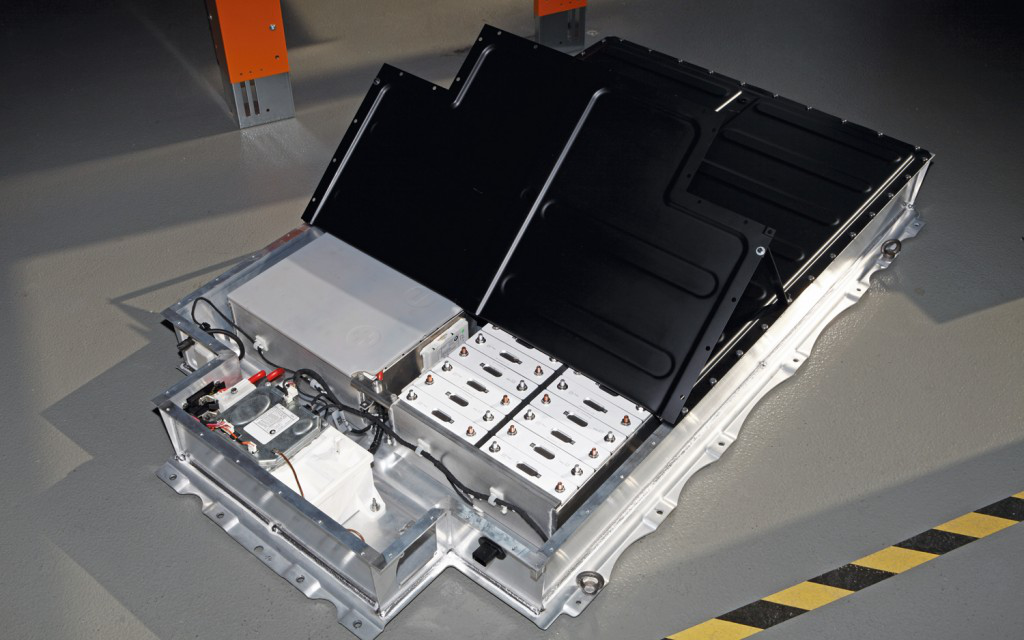
\includegraphics[width=1.0\columnwidth]{images/bmw-i3-battery-pack.png}
	\caption{Battery-Pack des BMW i3. Es sind zwei Batteriemodule zu sehen, die an ein gemeinsames Batteriemanagement angeschlossen sind. Im offenen Modul sind die prismatischen Batteriezellen zu erkennen \cite{bmwblog}.}
	\label{battery pack}
\end{figure}
\subsection{Elektrochemischer Vorgang}
Das Prinzip einer Batterie besteht in der Möglichkeit, von außen ein elektrisches Potential in Form von Elektronenüberschuss oder -mangel an den beiden Elektroden der Batterie anzulegen. Die Batterie beginnt dann, dieses elektrische Potential in ein chemisches Potential umzuwandeln. Dabei geben Atome an der Mangel-Elektrode ein Elektron ab und wandern als positives Ion in Richtung der Überschuss-Elektrode. Dort können sie wieder ein Elektron aufnehmen und sich in die Struktur einlagern. Wenn ein Verbraucher an den äußeren Stromkreis angeschlossen wird, reagiert die Batterie mit einer Rückreaktion. Die eingelagerten Atome geben ein Elektron ab und wandern zurück zu ihrer ursprünglichen Elektrode, in die sie sich unter Aufnahme des Elektrons wieder einlagern. Die Batterie entlädt sich und liefert dabei elektrischen Strom.
\begin{figure}[h]
	\centering
	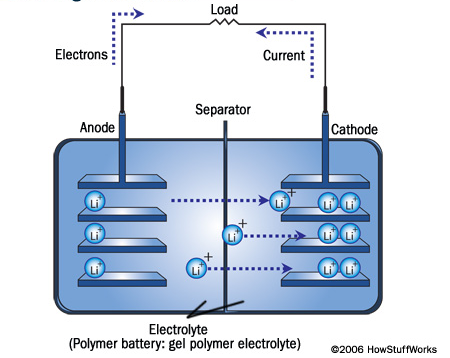
\includegraphics[width=0.7\columnwidth]{images/Schematischer_Aufbau_Li_Ionen.png}
	\caption{Schematischer Aufbau einer Li-Ionen-Batterie \cite{howstuffworks}.}
	\label{Li-Ionen_Batterie}
\end{figure}
\\\\
Im Falle einer \ce{LiFePO4}-Batterie mit graphitischer Anode wären die bei der Entladung ablaufenden Reaktionen \cite{minakshi2008book}:
\\\\
An der Anode:\\
\begin{equation}
	\ce{Li1C6 -> C6 + Li+ + e-}
\end{equation}
An der Kathode:\\
\begin{equation}
	\ce{Li+ + e- + FePO4 -> LiFePO4}
\end{equation}\\
Die Energie-  und Leistungsdichte von Batterien ist von einer Vielzahl verschiedener Mechanismen und Eigenschaften abhängig. Zunächst ist zwischen aktivem und restlichem Material innerhalb der Batterie zu unterscheiden. Komponenten wie der Separator, die Stromkollektoren, Binder und Leitruße, das Gehäuse oder auch ein ggf. existierendes Batteriemanagement sind elementare Bestandteile der Batterie. Sie dienen jedoch nicht direkt der Speicherung von Energie und senken so deren Diche im Verhältnis zum Gesamtgewicht der Batterie. Hier gilt es also, diese restlichen Komponenten möglichst gewichts- und raumsparend umsetzen zu können.
\\\\
\\ % Format-Fix
Auch die räumliche Struktur der Batterie hat einen entscheidenden Einfluss. Zum einen sollten die Elektroden relativ porös sein, um eine möglichst große Oberfläche zu besitzen und so eine größere Fläche zur Anlagerung bzw. Abgabe von Ionen zu bieten. Die sich einlagernden Teilchen sollten möglichst gut durch das Material zu Leerstellen hin diffundieren können. Der Fluss der Elektronen sollte mit wenig Widerstand funktionieren, da dieser einen Energie- und Leistungsverlust verursacht. Das Material sollte die neuen Atome so einlagern, dass sich seine ursprüngliche Struktur auch nach vielen Lade- und Entladevorgängen nicht zu stark verändert, da es sonst zur Alterung und damit Leistungsverringerung der Zelle kommt.   
%%% G: Festkoerperelektrolyt %%%
\section{Festkörperelektrolyten}
Da Flüssigelektrolyte verschiedene negative Eigenschaften aufweisen, bietet sich die Suche nach einer Alternative an. Hierbei sollen in der vorliegenden Arbeit Festkörperelektrolyte auf Basis von verschiedenen Keramiken untersucht werden. Diese müssen, um geeignet zu sein, Lithiumionen leiten können. Sie dürfen nicht elektronenleitend sein, um als Separator den Kurzschluss der Zelle zu verhindern. Sie müssen für einen gegebenen Temperaturintervall einen ähnlichen Wärmeausdehnungskoeffizient wie die restlichen Materialien der Zelle aufweisen. Bei der Anlagerung von Lithium zwecks Leitung darf sich ihr Volumen ebenfalls nicht zu stark ausdehnen. Eine besondere Herausforderung ist die Gestaltung der Grenzschicht zu den Elektroden. Die beiden Materialien müssen zueinander chemisch stabil sein. Die Grenzschichten müssen sich gut benetzen,n die Benetzung muss eine ausreichende Haftung aufweisen. Die Lithiumionen müssen an der Grenzschicht zwischen den unterschiedlichen Materialien wandern können.\\\\
Verschiedene Materialsysteme kommen potentiell für diese Aufgaben in Frage. Sie können grob anhand ihrer chemischen Struktur unterschieden werden.
\subsection{Perowskite}
\ce{LiLaTiO3} Typische ABO3-Struktur
\subsection{NASICON}
\ce{LiAlTi(PO4)3} Skelettartige Lampenstruktur
%%% G: NMR %%%
\section{NMR-Spektroskopie}
Die Grundlage der Kernspinresonanzspektroskopie (nuclear magnetic resonance spectroscopy, NMR-Spektroskopie) wurde zum Jahreswechsel 1945/1946 von zwei amerikanischen Forschungsgruppen unabhängig voneinander entwickelt. Felix Bloch und Edward M. Purcell wurden dafür 1952 mit dem Nobelpreis in Physik ausgezeichnet.
\\\\
\subsection{Physikalische Grundlagen der NMR-Spektroskopie}
Die NMR-Spektroskopie nutzt die magnetischen Eigenschaften von Atomkernen und ihren Umgebungen aus, um Aussagen über Zusammensetzungen und Bindungen von Stoffen treffen zu können.
\\\\
Elektronen, Neutronen und Protonen besitzen eine Eigenrotation, den Spin s. Der Spin eines Atomkerns setzt sich aus den Spins der einzelnen Protonen und Neutronen innerhalb des Kerns zusammen. Spins sind gequantelt und können daher nur gewisse diskrete Zustände annehmen. Dies gilt auch für den resultierenden Gesamtspin des Atomkerns. Die möglichen Zustände des Kernspins eines spezifischen Isotops können beschrieben werden über seine Spinquantenzahl I. Es existieren folgende magnetische Spinquantenzahlen m, welche die möglichen Orientierungen des Spins beschreiben:
\begin{equation}
m_I = I, I-1, I-2, ..., -I
\end{equation}
Die Gesamtzahl an möglichen Zuständen entspricht daher der Summe von 2I+1. Das Li$^7$ besitzt die Spinquantenzahl I=$\frac{3}{2}$. Es gilt daher:
\begin{equation}
m_{I=\frac{3}{2}} = \frac{3}{2}, \frac{1}{2}, -\frac{1}{2}, -\frac{3}{2}
\end{equation}
Sind in einem Atomkern die Anzahl an Protonen und Neutronen beide gerade, so gilt für die Spinquantenzahl I=0. Ein solcher Nukleus besitzt keinen Kernspin und kann daher nicht mittels NMR-Spektroskopie untersucht werden.
\\\\
Ein Atomkern besitzt eine Ladung. Wenn diese durch einen Kernspin bewegt wird, so besitzt der Nukleus ein magnetisches Moment $\mu$ in Abhängigkeit zum Zustand des Spins. Der Zusammenhang zwischen einem Drehmoment P und dem magnetischen Moment kann allgemein über das gyromagnetische Verhältnis $\gamma$ beschrieben werden: 
\begin{equation}
\mu = \gamma P
\end{equation}
Das Drehmoment des Kerns in Richtung z eines frei gewählten kartesischen Koordinatensystems entspricht dabei seiner magnetischen Spinquantenzahl multipliziert mit dem reduzierten Planckschen Wirkungsquantum:
\begin{equation}
P_z = m_I \hbar
\end{equation}
Das magnetische Moment kann also beschrieben werden mit:
\begin{equation}
\mu_z = \gamma m_I \hbar
\end{equation}
Keiner dieser möglichen Spinzustände ist energetisch günstiger als die anderen. Die Zustände liegen daher degeneriert vor. Dies kann allerdings durch das Anlegen eines starken äußeren Magnetfeldes B$_0$ in positiver z-Richtung beeinflusst werden. Es bilden sich verschiedene Energieniveaus für die unterschiedlichen Spinzustände aus. Die Energiedifferenz zwischen den Zuständen ist dabei proportional zur Stärke des angelegten äußeren Magnetfelds. Die Spins richten sich entlang der Achse aus. Die Energiediffernzen sind dabei für jeden Kern, der einen Spin besitzt, charakteristisch und können mit einer Frequenz in Abhängigkeit zur Stärke des äußeren Magnetfelds beschrieben werden. Diese Frequenz wird als Larmor-Frequenz bezeichnet und kann auch als Präzession des Kerns beschrieben werden.
\subsection{Aufbau eines NMR-Spektrometers}
\subsection{Betriebsmodus}
%\begin{equation}
%E = -\mu_z B_0
%\end{equation} 
\section{Kennzahlen}
\label{kennzahlen}
Um die später erzielten Ergebnisse besser einschätzen und vergleichen zu können, ist es nötig eine Reihe von Kennzahlen zu definieren, die bei der Einordnung und Charakterisierung unterschiedlicher Batteriezellen helfen \cite{jossen_2006}.
\begin{description}
\item[Nennladung] Die Nennladung ist als nutzbare Kapazität der Batterie definiert (mAh). Sie ist stark von der Art der Entladung abhängig.
\item[Energiedichte] Wird definiert als Verhältnis zwischen gespeicherter Energie und Volumen der Batterie (Wh/l). Wird statt des Volumens die Relation zur Masse angegeben, so spricht man von spezifischer Energie. 
\item[Leistungsdichte] Gibt äquivalent zur Energiedichte die vorhandene Leistung in Relation zum Volumen an (W/l). In Abhängigkeit zur Masse spricht man von spezifischer Leistung (W/kg).
\item[Lebensdauer] Definiert, ab wann ein gewisser Grad an Alterung erreicht ist. Normalerweise wird hier die Anzahl an Lade- und  Entladevorgängen genannt, bei der die Nennladung nicht unter 80\% der Ausgangsnennladung liegt.
\item[Ladezeit] Die Ladezeit kann zum einen absolut, also in Kapazität pro Stunde, oder aber relativ zur Nennladung auch in Prozent pro Stunde angegeben werden.
\end{description}

\newpage

\chapter{Strukturierung}
Es existieren verschiedene Verfahren zu Strukturierung des Aluminium-Stromkollektors. Diese, sowie die dabei zum Einsatz kommenden Maschinen sollen im Folgenden vorgestellt und diskutiert werden.
\section{Verwendete Materialien, Geräte und Maschinen}
Zum Einsatz kam eine Presse (WUM1) des Instituts für Mikrosystemtechnik. Diese kann über eine Software direkt angesteuert und programmiert werden. Dabei ist es möglich sowohl direkt Positionen anzufahren, als auch die Position über einen einstellbaren Druck bestimmen zu lassen. Weiterhin war es möglich die Presseinheit sowohl zu erhitzen, als auch über eine Wasserkühlung abzukühlen.\\\\
Es kamen Aluminiumfolien verschiedener Dicken sowie Teflonfolien und Polymethylmeth\-acrylatfolien (PMMA-Folien) zur Unterfütterung zum Einsatz. Die Formeinsätze wurden nach jeder Benutzung jeweils mit Ethanol gereinigt und vor der nächsten Benutzung mit einem Trennmittel (DexCoat8) behandelt.
\section{Prägen der Aluminiumfolie}
Für das Drucken und die Nanoprägelithografie waren keine passenden Geräte verfügbar. Beim Heißprägen wird eine bessere Verformbarkeit des zu strukturierenden Materials in der flüssigen bzw. geligen Phase ausgenutzt. Dies ist bei Aluminium allerdings erst bei sehr hohen Temperaturen möglich und daher nicht sinnvoll. Durchgeführt wurde daher das Kaltverformen sowie das Schleifen.
\subsection{Kaltverformen}
Beim Kaltverformen wird ein Formeinsatz mit hohem Druck in ein Substrat hineingepresst. Im Subtrat wird dadurch ein Negativ der im Formeinsatz vorhandenen Struktur erzeugt. Als Formeinsatz kam dabei ein bereits am IMT existierendes Modell zum Einsatz. \\\\
Der verwendete Formeinsatz wies vier baugleiche Strukturfelder auf, die quadratisch auf einem runden Substrat angebracht waren. Die Struktur selbst waren mehrere Millimeter lange Bahnen mit einer Tiefe von \SI{8}{\micro\meter} und einer Breite von \SI{2}{\micro\meter}. \\\\
Zunächst wurde der Formeinsatz auf der Presse angebracht. Er wurde mit einer \SI{750}{\micro\meter} dicken Aluminiumfolie und einer \SI{110}{\micro\meter} dicken Teflonfolie unterfüttert. Auf den Formeinsatz wird dann die zu strukturierende Aluminiumfolie aufgelegt. Diese wies eine Dicke von \SI{110}{\micro\meter} auf. Die Aluminiumfolie bedeckte dabei nicht den ganzen Formeinsatz, sondern wurde auf die Größe eines Strukturfeldes zurecht geschnitten. Als letzter Schritt wurde eine ebenfalls zurecht geschnittene PMMA-Folie auf der Aluminiumfolie angebracht. Der vollständige Aufbau wird in Abbildung \ref{schema_strukturierung} skizziert.
\begin{figure}[h]
	\centering
	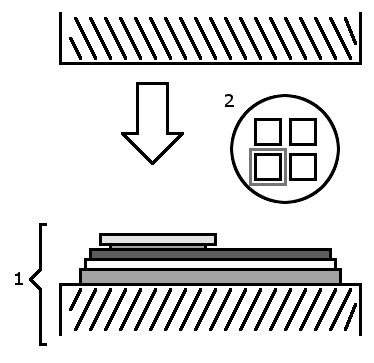
\includegraphics[width=0.7\columnwidth]{images/Schema_Strukturierung.jpg}
	\caption{Skizze des Versuchsaufbaus zur Strukturierung der Aluminiumfolie. 1 (von oben nach unten): PMMA-Folie, dünne Aluminiumfolie, Formeinsatz, Teflonfolie, dicke Aluminiumfolie, Pressvorrichtung; 2: Draufsicht auf den Formeinsatz mit markierten Strukturfeldern (schwarz) und Auflagefläche des Aluminiums (grau).}
	\label{schema_strukturierung}
\end{figure}
\\\\
Abbildung \ref{Al_Struktur} zeigt die fertig strukturierte Aluminiumfolie. Diese wurde anschließend noch mit einem Lichtmikroskop untersucht. Mit einer Fokusmessung konnte dabei die Tiefe der Struktur auf \SI{6}{\milli\meter} bei einer Breite von \SI{2}{\milli\meter} bestimmt werden. Das Aspektverhältnis der Probe beträgt daher 3:1.
\begin{figure}[h]
	\centering
	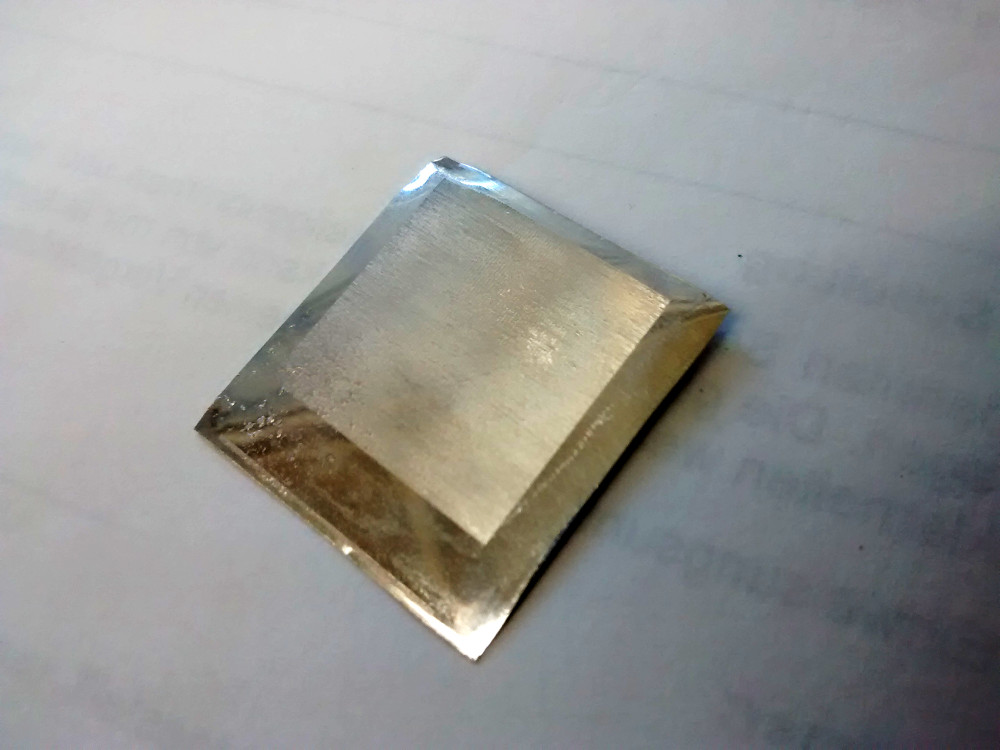
\includegraphics[width=0.85\columnwidth]{images/Al_Struktur.jpg}
	\caption{Mikrostrukturiertes Aluminium}
	\label{Al_Struktur}
\end{figure}
\subsection{Schleifen}
Das Schleifen beschreibt die gezielte Aufrauung der Oberfläche. Dieses Verfahren ist in der Umsetzung einfacher als das gezielte Strukturieren mittels Formeinsatz, bietet dafür aber auch weniger Kontrolle über das Ergebnis. Ein Beispiel ist das Sandstrahlen einer Oberfläche. \\\\
Zur Umsetzung im Rahmen dieser Arbeit wurde eine Aluminiumfolie mit einem sandgestrahlten Formeinsatz kaltverformt. Abbildung \ref{Formeinsatz_Sand} zeigt den benutzten Formeinsatz. 
Das so erzielte Negativ der aufgerauten Oberfläche des Formeinsatzes entspricht einer sandgestrahlten Aluminiumfolie.\\
\begin{figure}[h]
	\centering
	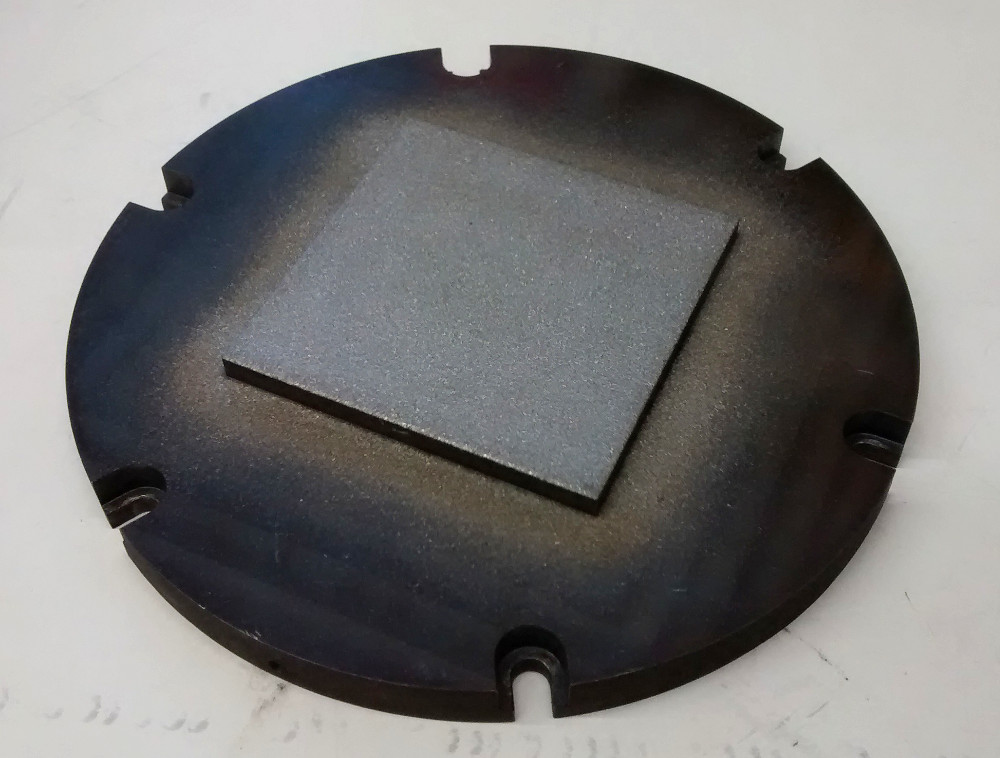
\includegraphics[width=0.85\columnwidth]{images/Formeinsatz_Sand.jpg}
	\caption{Formeinsatz zur Herstellung sandgestrahlter Oberflächen}
	\label{Formeinsatz_Sand}
\end{figure}
\chapter{Probenaufbau}
Um eine mögliche Verbesserung der Eigenschaften des strukturierten Stromkollektors in Batterien zu überprüfen, musste dieser zunächst in eine geeignete Testumgebung eingebaut werden. Weiterhin sind in dieser Testumgebung als Stromkollektor auch eine Probe auf Basis der unbearbeiteten Aluminiumfolie sowie eine Probe auf Basis der sandgestrahlte Aluminiumfolie eingebaut worden.
\section{Testzelle}
Als Testzelle kommt ein einfaches, gestapeltes Design, ähnlich einer Knopfzelle, zum Einsatz. Dies ist vollkommen ausreichend um die Grenzschicht zwischen Stromkollektor und Elektrode untersuchen zu können und erlaubt damit auch Aussagen über die Verbesserungsmöglichkeiten von gewickelten Zellen.
\subsection{Aufbau}
Die Testzelle besteht aus einem Glaszylinder mit einem Innendurchmesser von \SI{10}{\milli\meter} und einer Höhe von \SI{170}{\milli\meter}. An den beiden Enden des Zylinders befindet sich ein außenliegendes Gewinde. Dort kann ein Edelstahlstempel eingeführt werden. Der Stempel besitzt einen Hinterschnitt, welcher verhindert, dass er vollständig in den Zylinder rutschen kann. Mittels eines Plastikverschlusses mit innenliegendem Gewinde, welcher auf den Glaszylinder schraubbar ist, kann nun der Edelstahlstempel am Ende des Glaszylinders fixiert werden. Ein in einer Kerbe am Stempel fixierter Dichtungsring garantiert die Abdichtung der Zelle nach außen. Mittels einer simplen \SI{2}{\milli\meter}-Bohrung am Stempel kann dieser nach außen hin über einen Bananenstecker kontaktiert werden.\\\\
Innerhalb des Glaszylinders kommt zwischen Anode und Stempel eine Edelstahlfeder zum Einsatz. Diese garantiert den nötigen Anpressdruck und damit die vollständige Benetzung der Elektroden mit Elektrolyt sowie die Kontaktierung der Elektroden mit den Stempeln. Zur besseren Durckverteilung und Kontaktierung werden noch \SI{3}{\milli\meter} dünne Edelstahlplättchen an den außenliegenden Elektrodenseiten eingesetzt.\\\\
Eine Übersicht über den schematischen Aufbau der Testzelle ist in Abbildung \ref{schema_zelle} zu finden.
\begin{figure}[h]
	\centering
	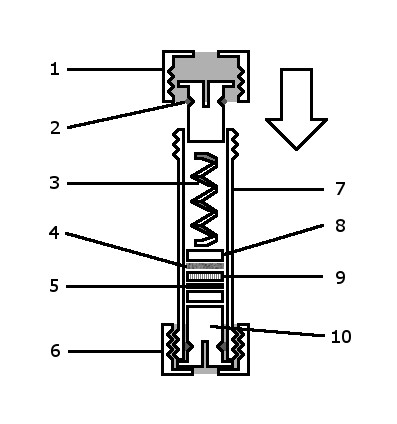
\includegraphics[width=0.7\columnwidth]{images/Schema_Zelle.jpg}
	\caption{Schema der Testzelle; 
			1: Plastikkappe,
			2: Dichtungsring,
			3: Edelstahlfeder,
			4: Kathode,
			5: Anode,
			6: Plastikkappe,
			7: Glaszylinder,
			8: Kontaktierplättchen,
			9: Separator,
			10: Edelstahlstopfen.
			}
	\label{schema_zelle}
\end{figure}
\subsection{Herstellung der fertigen Testzelle}
Die Testzellen müssen unter Schutzgasatmosphäre in einer Handschuhbox (siehe Abbildung \ref{handschuhbox}) gefertigt werden. Dies ist nötig, da sowohl das rein metallische Lithium, aber insbesondere auch der zum Einsatz kommende Flüssigelektrolyt mit dem Luftsauerstoff und der Luftfeuchtigkeit reagieren können. Als Flüssigelektrolyt kommt dabei das kommerzielle Produkt LP30 der Firma Merck zum Einsatz. Dieser besteht aus einem organischen Lösungsmittel, in dem verschiedene Lithiumsalze als Flourverbindungen gelöst sind. In Kontakt mit Luftfeuchtigkeit reagiert dieser und es entsteht hochätzende Flusssäure. 
\\\\
Für den Aufbau einer Testzelle wird ein Stempel in einen Glaszylinder eingeführt und mit einer Kappe fixiert. Anschließend kann die Zelle von der anderen Seite des Zylinders befüllt werden. Dafür wird zunächst ein Edelstahlplättchen und die Kathodenprobe eingesetzt. Darauf werden zwei Lagen Separator gelegt. Dadurch hat man die Sicherheit, dass selbst bei einem lokalen Defekt eines Separators immer noch das Verhindern des Kurzschlusses gewährleistet ist. Die Separatoren werden dann mit \SI{160}{\micro\litre} Elektrolyt benetzt. Nun kann die Lithiumanode und das obere Edelstahlplättchen abgelegt werden. Darauf wird die Feder gestellt und mit dem oberen Stempel und der oberen Kappe komprimiert sowie die Testzelle verschlossen.
\begin{figure}[h]
	\centering
	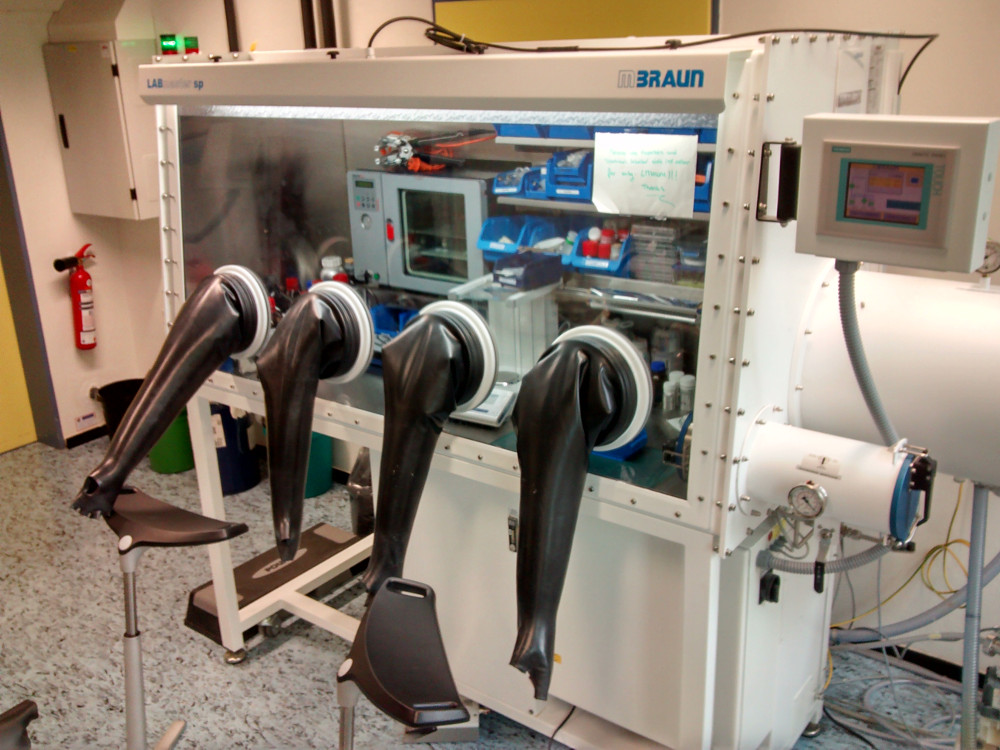
\includegraphics[width=1.0\columnwidth]{images/handschuhbox.jpg}
	\caption{Handschuhbox der Firma MBraun}
	\label{handschuhbox}
\end{figure}
\section{Herstellung der Kollektorproben}
Die hergestellten, strukturierten Folien müssen für den Einsatz als Stromkollektor innerhalb der Testzelle noch in die richtige Form gebracht werden. Dafür wurden diese mit einem runden Stanztool (\SI{10}{\milli\meter}) manuell zu Probenplättchen weiterverarbeitet. Diese Plättchen wurden anschließend gewogen. Dabei konnte ein Gewicht von \SI{24.3 \pm 0.2}{\milli\gram} festgestellt werden.
\section{Herstellung des Aktivmaterials}
An den beiden Elektroden der Testzelle kommt reines Lithium sowie eine \ce{LiCoO2}-Mischung zum Einsatz. Der Batterie funktioniert über eine Interkalation des Lithiums. Die ablaufenden Reaktionen beim Entladen der Zelle sind daher gegeben mit \cite{bub_skript}: \\\\
\\%Unschöner Fix für Umbruchproble :-p
An der Anode:\\
\begin{equation}
	\ce{3Li ->  3Li+ + 3e-}
\end{equation}
An der Kathode:\\
\begin{equation}
	\ce{3Li+ + 3e- + 5(Li_{0,4}CoO2)^{-0,6} -> 5LiCoO2}
\end{equation}
Wichtig ist hier, dass das Aktivmaterial nicht vollständig entladen werden darf, da es ansonsten zu einem Zusammenbruch der $\ce{CoO2}$-Schichten kommt. Dies führt zur Entstehung von Sauerstoff, welcher im schlimmsten Fall in der Lage ist die Zelle zu sprengen. Daher dürfen Zellen mit \ce{LiCoO2}-Kathode nur bis zu einer Ladeschlussspannung von \SI{4.2}{\volt} geladen werden \cite{bub_skript}.
\subsection{Lithium-Anode}
Als Anode wurde in den Testzellen reines Lithium eingesetzt. Dieses besitzt eine ausreichend gute elektrische Leitfähigkeit von \SI{10.6e6}{\siemens\per\meter} \cite{binder1999lexikon} und muss daher weder im Material selbst noch über einen Stromkollektor speziell kontaktiert werden, sondern kann direkt mit dem Anodenstempel der Testzelle verbunden werden. Lithium lagert weiteres Lithium perfekt ein und besitzt ein hervoragendes Halbzellenpotential. Es besitzt allerdings Nachteile in der Sicherheit sowie der Langzeitstabilität. Dies ist in den Testzellen jedoch vernachlässigbar, da diese nicht auf einen dauerhaften Einsatz hin untersucht werden.
\\\\
Das Ausgangsmaterial ist dabei kommerziell erhältliche Lithiumfolie (Sigma Aldrich), welche unter Schutzgasatmosphäre in einer Handschuhbox gelagert und verarbeitet wird. Dies ist nötig, da Lithium sehr reaktiv gegenüber Wasser ist und unter Sauerstoff eine passivierende Oxidschicht bildet. Als weiches Leichtmetall lässt es sich gut bearbeiten. Daher ist es möglich, es in der Handschuhbox mit einer händisch betriebenen Walzenpresse auf eine geeignete Dicke zu walzen. Lithium wird in den Zellen immer im Überschuss vorgelegt um einen vollständigen Abbau zu verhindern. Die gewalzte Folie kann dann in der Handschuhbox mit einem einfachen Stanzwerkzeug unter manuellem Druck zu runden Anodenplättchen weiterverarbeitet werden.
\subsection{\ce{LiCoO2}-Kathode}
Auf Kathodenseite kommt ein \ce{LiCoO2}-Slurry zum Einsatz. Dieses Material wird seit über 30\;Jahren in kommerziellen Batteriezellen eingesetzt und ist gut untersucht. Das Anodenmaterial besteht dabei aus einer Mischung von \SI{45}{\masspercent} \ce{ LiCoO2},  \SI{45}{\masspercent} Leitruß und  \SI{10}{\masspercent} kommerzieller Binder. Diese Stoffe werden mit einem organischen Lösungsmittel wie Isopropanol vermischt. Dabei entsteht der viskose Slurry, der auf den Stromkollektor aufgetragen werden kann. Dies geschieht manuell mit Hilfe eines Spatels direkt auf die vorher gestanzten Kollektorproben. Die so hergestellten Proben werden zum Trocknen 24\;Stunden lang unter einem Abzug gelagert. Dabei entweicht das noch im Slurry vorhandene Lösungsmittel und die Probe wird fest.
\begin{figure}[]
	\centering
	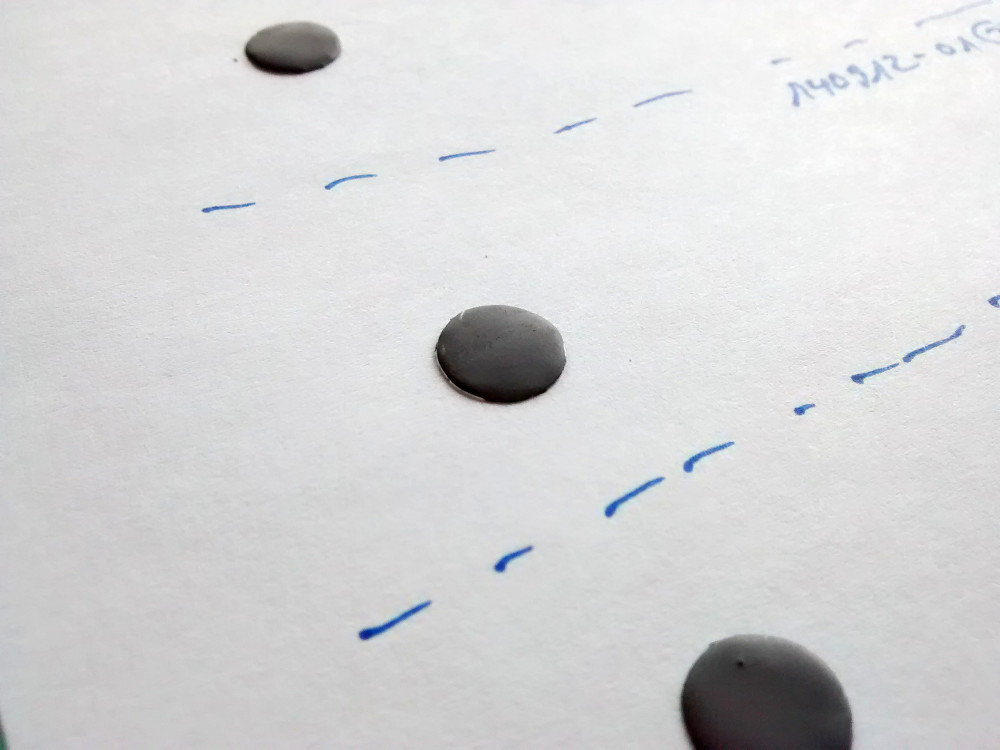
\includegraphics[width=1.0\columnwidth]{images/Kathodenprobe.jpg}
	\caption{Hergestellte Kathodenproben (10mm Durchmesser)}
	\label{kathodenproben}
\end{figure}
Anschließend müssen die so hergestellten Kathodenproben noch gewogen werden. Durch das Gewicht ist sowohl die Aktivmasse als auch die Höhe des aufgetragenen Kathodenmaterials (KM) berechenbar. Dabei gilt:
\begin{equation}
\begin{split}
\rho_{KM} &= 0,45 \rho_{\ce{LiCoO2}} + 0,45 \rho_{Ruß} + 0,1 \rho_{Binder} = 3,24 \frac{g}{cm^3}\\\\
A_{Probe} &= 2 \pi r^2 = 1,571cm^2  \\\\
h_{KM} &= \frac{V_{KM}}{A_{Probe}} = \frac{\frac{m_{KM}}{\rho_{KM}}}{A_{Probe}} =  \frac{m_{KM}}{5,09g}cm\\\\
\end{split}
\end{equation}
Dabei kann die Masse des Kathodenmaterials aus der Massendifferenz von Stromkollektor und Gesamtprobe bestimmt werden. Die Aktivmasse innerhalb der Kathode ergibt sich aus dem Produkt von 0,45 und der Masse des Kathodenmaterials. Die so bestimmten Werte lassen sich in Tabelle \ref{tabelle_massen} finden
\begin{table}[h]
\begin{tabular}{lllll}
\toprule
 & & \textbf{Masse Probe} & \textbf{Masse KM} & \textbf{Höhe KM}\\
\midrule
\multirowbt{3}{*}{\textbf{Probe}} & \textit{Reines Aluminium} & \quad \SI{32.9}{\milli\gram} & \quad  \SI{8.6}{\milli\gram}  & \quad \SI{169}{\micro\meter}\\
\cmidrule{2-5}
 & \textit{Sandgestrahltes Aluminium} & \quad  \SI{29.0}{\milli\gram} & \quad  \SI{4.7}{\milli\gram} & \quad \, \SI{92}{\micro\meter}\\
\cmidrule{2-5}
 & \textit{Strukturiertes Aluminium} & \quad  \SI{27.1}{\milli\gram} & \quad  \SI{2.8}{\milli\gram} &\quad \, \SI{55}{\micro\meter}\\
\bottomrule
\end{tabular}
 \caption{Massen und Höhen der unterschiedlichen Proben.}
 \label{tabelle_massen}
 \end{table} 
 \\\\
Die Ursache für die stark unterschiedlichen Schichtdicken konnte dabei nicht ermittelt werden. Da in allen Fällen jedoch eine vollständige Benetzung des Kollektors stattgefunden haben sollte, ist dies für die Untersuchung der Grenzschicht zwischen Kollektor und Aktivmaterial unerheblich. Auf ein Kalandrieren der Probe wurde verzichtet.

\chapter{Diskussion der Ergebnisse}
\label{discussion}
Im Folgenden werden die aus den Testzellen erhaltenen Daten vorgestellt und diskutiert. Dabei kommt als Methode vor allem die Impedanzspektroskopie zum Einsatz.
\section{Relevante Kennzahlen}
In Abschnitt \ref{kennzahlen} wurden verschiedene Kennzahlen für Batterien eingeführt. Es kann zunächst bestimmt werden, welche dieser Kennzahlen von einer Strukturierung des Stromkollektors beeinflusst werden.
\begin{description}
\item[Nennladung] Die Nennladung ist lediglich von den eingesetzten Aktivmaterialien abhängig, da diese die Anzahl an lagerfähigen Ladungen bestimmen.
\item[Energiedichte] Durch eine Verringerung der Verluste beim Ladungstransport zwischen Aktivmaterial und Stromkollektor kann die Zelle eine höhere Energie liefern.
\item[Leistungsdichte] Ein geringerer Widerstand beim Ladungstransport zwischen Aktivmaterial und Stromkollektor erhöht die Leistungsdichte der Batterie.
\item[Lebensdauer] Die Lebensdauer könnte von einer besseren Struktur profitieren. Jedoch sind Versuche in diesem Bereich sehr langwierig und wurden daher nicht durchgeführt.
\item[Ladezeit] Die Geschwindigkeit, mit der eine Zelle geladen werden kann, ist sehr stark abhängig von der Diffusionsgeschwindigkeit der Lithiumionen innerhalb der Aktivmaterialien. Hier ist keine Verbesserung zu erwarten.
\end{description}
Als relevante Kennzahlen können also die Energie- sowie die Leistungsdichte benannt werden. Bei beiden ist dabei die Verringerung der Verluste beim Ladungstransport zwischen Aktivmaterial und Stromkollektor die entscheidende Größe. Diese Verlustmechanismen können besonderds gut mittels einer elektrochemischen Impedanzspektroskopie detektiert werden.
\section{Batterietests}
Zum Testen der Batterien wurden diese zunächst vollkommen geladen. Dabei wurde auf eine gezielte Formierung der Zellen verzichtet. Anschließend wurde die Leerlaufspannung bestimmt und eine Impedanzspektroskopie durchgeführt.
\subsection{Impedanzspektroskopie}
Die Impedanzspektroskopie nutzt aus, dass kapazitive und induktive Bauelemente in der Elektrotechnik einen sich über den Zeitverlauf ändernden Widerstand besitzen. Bei einem Wechselstrombetrieb spricht man dabei von einem komplexen, frequenzabhängigen Widerstand. Diese Wiederstände sind allerdings auch von weiteren externen Faktoren wie der Temperatur und dem Ladezustand der Batterie abhängig. Eine weiterführende Einleitung und Diskussion lässt ist in \cite{schmidt2013verfahren} zu finden.
\begin{figure}[h]
	\centering
	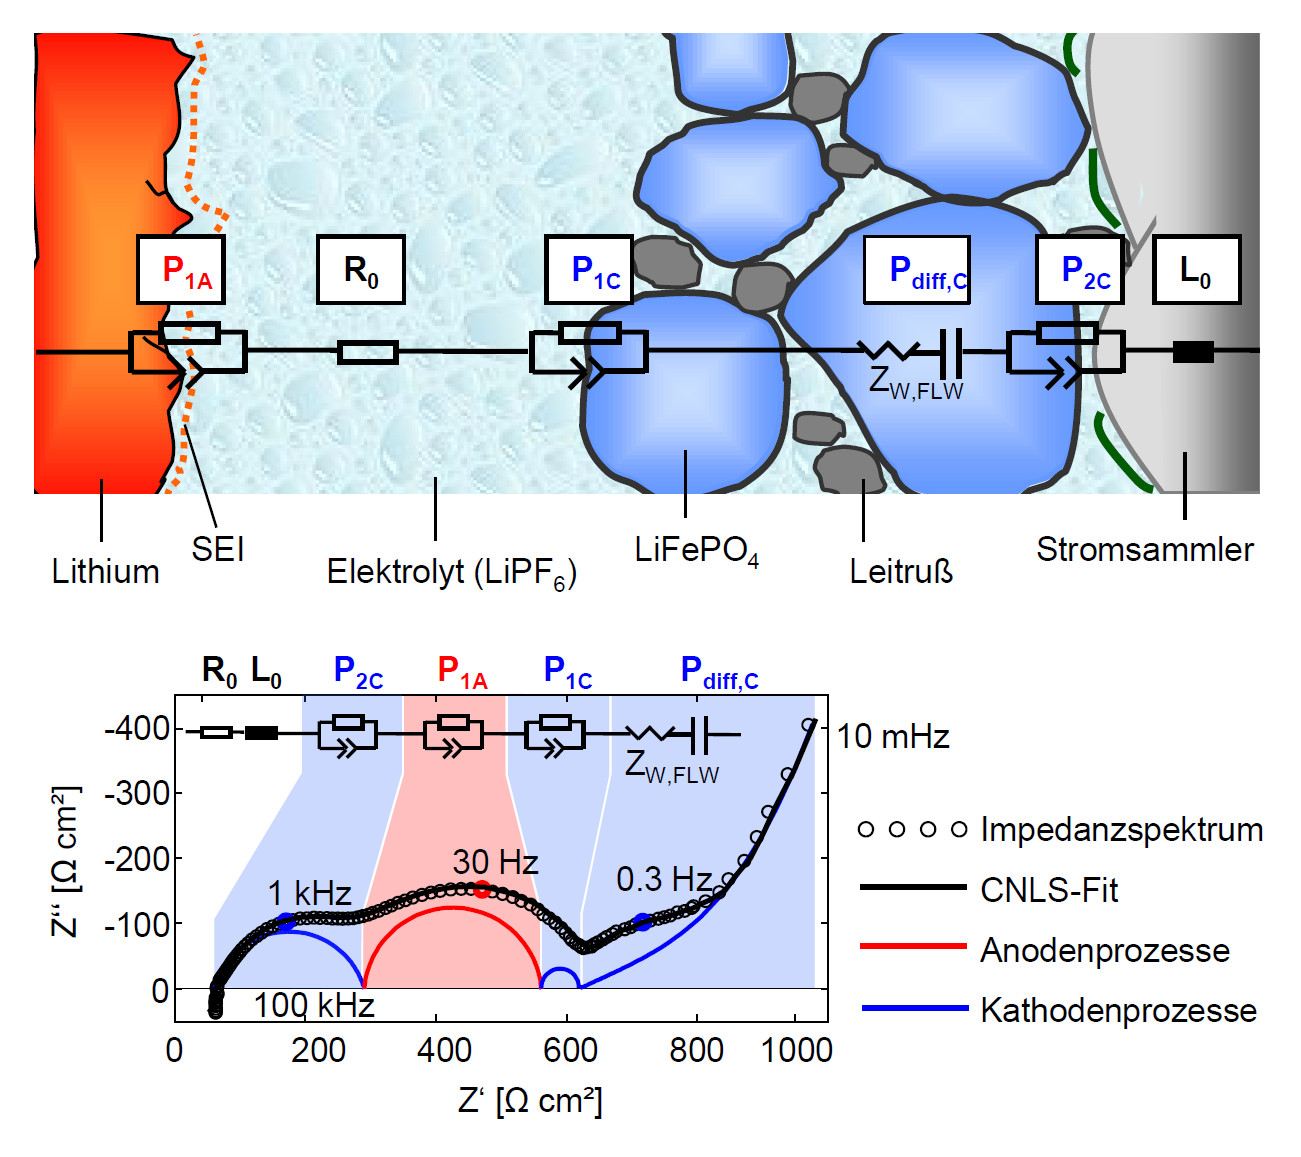
\includegraphics[width=1.0\columnwidth]{images/Schema_IS.jpg}
	\caption{Detektierung unterschiedlicher Verlustmechanismen verschiedener Grenzschichten innerhalb einer \ce{LiFePO4}-Zelle mittels Impedanzspektroskopie \cite{bub_skript}.}
	\label{schema_is}
\end{figure}
\subsubsection{Elektrochemisches Ersatzschaltbild}
Eine Batteriezelle besitzt unterschiedliche Verlustmechanismen, die mit einem elektrochemischen Ersatzschaltbild modelliert werden können. Abbildung \ref{schema_is} zeigt hier das Ersatzschaltbild für eine Lithium-\ce{LiFePO4}-Zelle. Interessant sind hierbei die kathodenseitigen Mechanismen. Diese laufen für den Übergang zwischen Kathode und Stromkollektor bei niedrigen Frequenzen um \SI{1}{\kilo\hertz} ab.
\subsubsection{Nyquist-Plot}
Der Nyquist-Plot ist eine Möglichkeit der Darstellung der Ergebnisse einer Impedanz\-spek\-troskopie-Messung. Dabei werden Real- und Imaginärteil des Widerstands einer Zelle aufgetragen. Die einzelnen Punkte entsprechen dabei einer bestimmten Frequenz. Verschiedene elektrotechnische Bauteile stellen sich unterschiedlich dar. So ist ein einfacher realer Widerstand lediglich ein Punkt auf der realen Achse. Induktive und kapazitive Elemente stellen sich als Linien parallel zur imaginären Achse dar. Die Parallelschaltung von Widerstand und Kondensator (RC-Glied) ist ein Halbkreis auf der realen Achse, ein RQ-Glied ein abgeflachter Halbkreis. Diffusionsbewegungen können mit sogenannten Wartburg-Elementen dargestellt werden, welche eine \ang{45}-Steigung aufweisen.
\subsubsection{Linearer Kramers-Kronig Test}
Messungen von Impedanzspektren sind sehr fehleranfällig. Eine Methode um die Validität eines Spektrums zu bestimmen, ist der lineare Kramers-Kronig Test \cite{schonleber2014method}. Auf Basis dieses Testes stellt das Institut für angewandte Materialien - Werkstoffe der Elektrotechnik (IAM-WET) auf ihrer Internetseite das Programm Lin-KK zur Verfügung, mit welchem für eine distinkte Anzahl an RC-Gliedern ein nach dem Kramers-Kronig Test idealer Fit für die gegebenen Impedanzdaten gefunden werden kann. 
\subsection{Ergebnisse}
Die Daten der Impedanzspektroskopie zwischen den verschiedenen Proben unterscheiden sich teilweise. Neben den unterschiedlichen Schichtdicken könnte dies auch an teilweise abweichenden Ladezuständen sowie an der Formierung der Zellen liegen. Diese Faktoren beeinflussen hauptsächlich die Grenzfläche zwischen den Elektroden und dem Elektrolyt sowie den Mechanismen innerhalb der Aktivmaterials. Die Grenzfläche zwischen Stromkollektor und Kathode sollte jedoch nur im geringeren Maße davon beeinflusst sein.
\\\\
Die Abbildungen \ref{plot_rein}, \ref{plot_sand} und \ref{plot_struktur} zeigen die durchgeführten Impedanzmessungen sowie den darin gefundenen Anteil der Grenzschicht zwischen Kathode und Stromkollektor an den Verlustmechanismen als angefitteter Halbkreis. Dessen Durchmesser entspricht dem Widerstand der Grenzschicht \cite{bub_skript}. Eine Übersicht über die so ermittelten Widerstände lässt sich in Tabelle \ref{tabelle_is} finden.
\\\\
Es ist zu erkennen, dass sich der Widerstand der Grenzfläche bei einem unstrukturierten Stromkollektor kaum von dem des strukturierten unterscheidet. Die sandgestrahlte Oberfläche hingegen weist einen deutlich geringeren Widerstand auf. Eine mögliche Erklärung für dieses Verhalten wäre eine unvollständige Benetzung der Struktur durch das Aktivmaterial. Sollten die Kavitäten nur unzureichend gefüllt werden, so entstehen funktionslose Hohlräume zwischen Kollektor und Aktivmaterial. Dies erklärt auch das bessere Abschneiden der sandgestrahlten Struktur, welche durch die deutlich gröbere Struktur größere Kavitäten besitzt.
\begin{figure}[h]
\centering
\begin{tikzpicture}[thick, scale=1.0]
	\begin{axis}[
		clip mode=individual, %lines above marks
		% title =  \textbf{\large{Testtitel}},
		legend style = {draw=none},
		%legend pos = outer north east,
		xlabel = {$Z' [\Omega]$},
		xmax = 120,
		xmin = 0,
		xtick={10,20, 30,40, 50, 60, 70, 80, 90, 100, 110},
 		%x tick label style={/pgf/number format/1000 sep=},
		ylabel =  {$Z'' [\Omega]$},
		ymax = 0,
		ymin = -60,
		ytick={0, -10,-20,-30,-40, -50},
		y dir = reverse,
		%x dir = reverse,
		scale only axis, % The height and width argument only apply to the actual axis
		height=6cm,
		width = 12cm,
		%width=\textwidth-\widthof{100}-5.0cm, % \textwidth minus width of longest label text minus label offset
		yticklabel style={align=left,inner sep=5pt,xshift=-0.1cm}, % No inner sep, to remove whitespace on left, manually offset by given distance
		%xticklabel style={align=top,inner sep=5pt,xshift=-0.1cm}
		]

		\addplot[
			color = black,
			%fill = black,
			mark = *, % * = leer
			%only marks
			smooth,
			]
 		coordinates {
( 13.35491372 , -0.563650555 )
( 13.14612673 , -0.984618131 )
( 13.06691664 , -1.718507665 )
( 13.20067476 , -2.774256004 )
( 13.6528094 , -4.175149534 )
( 14.58397755 , -5.898781609 )
( 16.12033774 , -7.779986906 )
( 18.14749962 , -9.601290538 )
( 20.29958981 , -11.44612662 )
( 22.45900976 , -13.88615245 )
( 25.09613975 , -17.54878373 )
( 29.26666543 , -22.64616393 )
( 36.34203507 , -28.48123923 )
( 46.90834146 , -32.91293275 )
( 59.38976526 , -33.50521596 )
( 70.62328956 , -29.95056847 )
( 78.41846615 , -24.55429273 )
( 83.19111503 , -19.63882714 )
( 86.28020923 , -16.22348437 )
( 88.90431352 , -14.21315355 )
( 91.69800599 , -12.93738051 )
( 94.54304202 , -11.7177842 )
( 96.94756866 , -10.4597305 )
( 98.72853615 , -9.596668383 )
( 100.2180044 , -9.512150813 )
( 101.955546 , -10.27295226 )
( 104.4207079 , -11.53035609 )
( 107.738174 , -12.63113329 )
( 111.3117898 , -13.09867158 )
( 114.4538577 , -13.27691613 )
( 117.1740049 , -13.98298967 )
( 120.2067809 , -15.72471217 )
( 124.7128133 , -18.28560204 )
( 131.637456 , -20.35490246 )
( 140.6379313 , -19.7455131 )
			};

		\addlegendentry{Lin-KK Fit}

		\addplot[
			color = red,
			%fill = black,
			mark = none, % * = leer
			%only marks
			ultra thick,
			smooth,
			]
 		coordinates {
( 26.70357819 , -1.391502867 )
( 25.78956979 , -4.802628633 )
( 23.29245242 , -7.299746005 )
( 19.88132665 , -8.213754399 )
( 16.47020089 , -7.299746005 )
( 13.97308352 , -4.802628633 )
( 13.05907512 , -1.391502867 )
			};

		\addlegendentry{2C}
	\end{axis}
\end{tikzpicture}
\caption{Impedanz\-spektroskopie der Probe mit unbehandeltem Aluminium-Strom\-kol\-lek\-tor.}
\label{plot_rein}
\end{figure}

\begin{figure}[h]
\centering
\begin{tikzpicture}[thick, scale=1.0]
	\begin{axis}[
		clip mode=individual, %lines above marks
		% title =  \textbf{\large{Testtitel}},
		legend style = {draw=none},
		%legend pos = outer north east,
		xlabel = {$Z' [\Omega]$},
		xmax = 120,
		xmin = 0,
		xtick={10,20, 30,40, 50, 60, 70, 80, 90, 100, 110},
 		%x tick label style={/pgf/number format/1000 sep=},
		ylabel =  {$Z'' [\Omega]$},
		ymax = 0,
		ymin = -60,
		ytick={0, -10,-20,-30,-40, -50},
		y dir = reverse,
		%x dir = reverse,
		scale only axis, % The height and width argument only apply to the actual axis
		height=6cm,
		width = 12cm,
		%width=\textwidth-\widthof{100}-5.0cm, % \textwidth minus width of longest label text minus label offset
		yticklabel style={align=left,inner sep=5pt,xshift=-0.1cm}, % No inner sep, to remove whitespace on left, manually offset by given distance
		%xticklabel style={align=top,inner sep=5pt,xshift=-0.1cm}
		]

		\addplot[
			color = black,
			%fill = black,
			mark = *, % * = leer
			%only marks
			smooth,
			]
 		coordinates {
( 16.2699996 , -0.292245891 )
( 16.18739661 , -1.001885264 )
( 16.25588309 , -1.949536819 )
( 16.58446136 , -3.162590838 )
( 17.29969648 , -4.622070471 )
( 18.49086406 , -6.219465885 )
( 20.0766897 , -7.833100659 )
( 21.88148423 , -9.588481539 )
( 23.99506989 , -11.85309387 )
( 26.99992711 , -14.84125937 )
( 31.64269055 , -18.07583694 )
( 38.09953615 , -20.31383789 )
( 45.26133189 , -20.42279354 )
( 51.35143513 , -18.73617739 )
( 55.77190569 , -16.70312954 )
( 59.19633095 , -15.35078665 )
( 62.48734316 , -14.75908632 )
( 66.03946595 , -14.34006635 )
( 69.48264999 , -13.69439252 )
( 72.40188991 , -13.12471667 )
( 74.99216452 , -13.18733934 )
( 77.9024224 , -13.99950358 )
( 81.64712763 , -15.02040836 )
( 85.95676708 , -15.45649779 )
( 89.97320673 , -15.18572134 )
( 93.1561243 , -14.96580821 )
( 95.79727152 , -15.61030882 )
( 98.6201391 , -17.37515211 )
( 101.9953155 , -19.9656405  )
( 105.6407428 , -23.17961296 )
( 109.0194718 , -27.64327698 )
( 112.1485204 , -34.61125466 )
( 115.7833941 , -45.4045863  )
( 120.7067102 , -60.89574462 )
( 126.8350451 , -81.97223071 )
			};

		\addlegendentry{Lin-KK Fit}

		\addplot[
			color = red,
			%fill = black,
			mark = none, % * = leer
			%only marks
			ultra thick,
			smooth,
			]
 		coordinates {
( 25.05136513 , -1.157987011 )
( 24.45740767 , -3.37466641 )
( 22.83468573 , -4.997388354 )
( 20.61800633 , -5.591345808 )
( 18.40132693 , -4.997388354 )
( 16.77860498 , -3.37466641 )
( 16.18464753 , -1.157987011 )
			};

		\addlegendentry{2C}
	\end{axis}
\end{tikzpicture}
\caption{Impedanz\-spektroskopie der Probe mit sand\-gestrahltem Aluminium-Strom\-kol\-lek\-tor.}
\label{plot_sand}
\end{figure}

\begin{figure}[h]
\centering
\begin{tikzpicture}[thick, scale=1.0]
	\begin{axis}[
		clip mode=individual, %lines above marks
		% title =  \textbf{\large{Testtitel}},
		legend style = {draw=none},
		%legend pos = outer north east,
		xlabel = {$Z' [\Omega]$},
		xmax = 120,
		xmin = 0,
		xtick={10,20, 30,40, 50, 60, 70, 80, 90, 100, 110},
 		%x tick label style={/pgf/number format/1000 sep=},
		ylabel =  {$Z'' [\Omega]$},
		ymax = 0,
		ymin = -60,
		ytick={0, -10,-20,-30,-40, -50},
		y dir = reverse,
		%x dir = reverse,
		scale only axis, % The height and width argument only apply to the actual axis
		height=6cm,
		width = 12cm,
		%width=\textwidth-\widthof{100}-5.0cm, % \textwidth minus width of longest label text minus label offset
		yticklabel style={align=left,inner sep=5pt,xshift=-0.1cm}, % No inner sep, to remove whitespace on left, manually offset by given distance
		%xticklabel style={align=top,inner sep=5pt,xshift=-0.1cm}
		]

		\addplot[
			color = black,
			%fill = black,
			mark = *, % * = leer
			%only marks
			smooth,
			]
 		coordinates {
( 18.54921609 , -0.166921257 )
( 18.5253482 , -0.778752491 )
( 18.57271384 , -1.546591828 )
( 18.75295754 , -2.545432976 )
( 19.16629634 , -3.845448808 )
( 19.96195832 , -5.465589332 )
( 21.25960033 , -7.305448278 )
( 22.98435939 , -9.231436459 )
( 24.86789206 , -11.37097487 )
( 26.88041297 , -14.27510527 )
( 29.53838427 , -18.53320418 )
( 33.93840781 , -24.33893402 )
( 41.52094409 , -30.95516585 )
( 52.9005946 , -36.11120632 )
( 66.38452301 , -37.23672593 )
( 78.59827535 , -34.07311509 )
( 87.25393107 , -29.1702974 )
( 92.94374059 , -25.09770813 )
( 97.35141133 , -22.92894706 )
( 102.0785625 , -22.3093561 )
( 107.8633756 , -21.93842718 )
( 114.0312994 , -20.52132146 )
( 119.1909376 , -18.03783121 )
( 122.6820945 , -15.60351252 )
( 124.9289534 , -14.20250091 )
( 126.6697261 , -14.25935005 )
( 128.5175009 , -15.73834505 )
( 130.7548301 , -18.45154819 )
( 133.1577898 , -22.43645138 )
( 135.4580451 , -28.45432476 )
( 137.8956743 , -37.85194754 )
( 141.310426 , -51.99315695 )
( 147.0263576 , -72.26370551 )
( 156.1554189 , -99.43922616 )
( 168.1503775 , -134.3570926 )
			};

		\addlegendentry{Lin-KK Fit}

		\addplot[
			color = red,
			%fill = black,
			mark = none, % * = leer
			%only marks
			ultra thick,
			smooth,
			]
 		coordinates {
( 32.26485886 , -0.740362387 )
( 31.34447898 , -4.175266869 )
( 28.82995438 , -6.689791468 )
( 25.3950499 , -7.61017135 )
( 21.96014541 , -6.689791468 )
( 19.44562081 , -4.175266869 )
( 18.52524093 , -0.740362387 )
			};

		\addlegendentry{2C}
	\end{axis}
\end{tikzpicture}
\caption{Impedanzspektroskopie der Probe mit mikrostrukturiertem Aluminium-Strom\-kollektor.}
\label{plot_struktur}
\end{figure}

\begin{table}[h]
\begin{tabular}{llll}
\toprule
 & & \textbf{Innerer Widerstand} & \textbf{Widerstand 2C}\\
\midrule
\multirowbt{3}{*}{\textbf{Probe}} & \textit{Reines Aluminium} & \quad \SI{13.1}{\ohm}  &  \quad \SI{13.6}{\ohm}\\
\cmidrule{2-4}
 & \textit{Sandgestrahltes Aluminium} & \quad \SI{16.2}{\ohm} & \quad \: \SI{8.9}{\ohm} \\
\cmidrule{2-4}
 & \textit{Strukturiertes Aluminium} & \quad \SI{18.5}{\ohm} & \quad \SI{13.7}{\ohm} \\
\bottomrule
\end{tabular}
 \caption{Ermittelte Widerstände der einzelnen Proben.}
 \label{tabelle_is}
 \end{table} 
\section{Wirtschaftlichkeit}
Die experimentell erreichten Ergebnisse lassen darauf schließen, dass eine Zellfertigung mit Strukturierung des Stromkollektors nicht als disruptive, sondern als kontinuierliche Innovation zu sehen ist \cite{bower1995disruptive}. Die zu erwartenden Leistungszugewinne sind nicht ausreichend um neue Einsatzgebiete zu ermöglichen. Daher muss sich ein gegebenenfalls neu zu etablierender Prozess gegen bereits existierende Prozesse durchsetzen.
\\\\
Momentan werden in Deutschland Produktionskosten von 380\euro pro kWh in der Batterie gespeicherter Energie erreicht \cite{fortschrittsbericht_npe}. Bei einer Verbesserung der Energiedichte um kleine Beträge, wie dies bei einer kontinuierlichen Innovation zu erwarten ist, dürfen die anfallenden Kosten daher nicht die zu erwartende Rendite übertreffen. Die Verbesserung der Batterie um 1\% bei der Energiedichte ist also mit Kosten von maximal 3,80\euro pro hergestellter Kilowattstunde Batterie in der Produktion zu realisieren. Für die Batterie eines BMW i3 von \SI{18.8}{\kWh} \cite{bmw_i3} würde dies maximale Mehrkosten von 71,44\euro pro Batterie bedeuten.
\\\\
Mit einem Pressen der Aluminiumfolien über eine große Presse, wie dies für die Proben angewandt wurde, ist ein solch enger Kostenrahmen nicht zu erreichen. Sollte die Strukturierung allerdings innerhalb einer Roll-to-Roll-Anlage stattfinden können, vorgelagert zum Coaten und Trocknen der Elektrodenfolie, so wäre dies denkbar. Jedoch muss hier eine ausreichend schnelle Strukturierung gewährleistet werden. In aktuellen Prozessen werden bereits 25-35m Folie pro Minute erreicht, erste Forschungsprojekte konnten bereits Geschwindigkeiten von bis zu 100m pro Minute zeigen \cite{kit_rekord_100m}. Für eine genauere Berechnung des Kostenrahmens sind hierzu insbesondere weitergehende Untersuchungen zur exakten quantitativen Verbesserung der Energiedichte notwendig.
\\\\
Da die Batteriesysteme bei modernen Elektromobilen einen Anteil an der Wertschöpfung von bis zu 40\% haben \cite{fortschrittsbericht_npe}, sind auch bei kleineren Effizienzzugewinnen im Prozess größere Investitionskosten in die zu verwendenden Anlagen  bei ausreichend hoher Laufzeit grundsätzlich zu rechtfertigen.
%\section{Vergleich mit der Literatur}
%?
\newpage

\chapter{Fazit}
Abschließend werden die wichtigsten Erkenntnisse dieser Arbeit noch einmal kurz zusammengefasst und mögliche Verbesserungs- und Veränderungsvorschläge in einem Ausblick gegeben.
\section{Zusammenfassung}
Die Herstellung gezielt strukturierter Aluminiumfolien mit mikrostrukturierter und sandgestrahlter Oberfläche für den Einsatz in Batteriezellen ist möglich. Diese konnten zu Elektrodenplättchen weiterverarbeitet werden. Die Elektrodenplättchen wurden erfolgreich in Batterietestzellen eingebaut und konnten über mehrere Zyklen hinweg getestet werden.
\\\\
Mittels Impedanzspektroskopie konnten die Proben anschließend auf ihren Wiederstand zwischen Aktivmaterial und Aluminiumfolie hin untersucht werden. Dabei wurde festgestellt, dass nur die sandgestrahlte Oberfläche ein verbessertes Verlustverhalten aufwies. 
\\\\
Eine wirtschaftliche Produktion von Batterien mit strukturierten Stromkollektorfolien ist denkbar. Es wird allerdings noch eine genauere, quantitative Untersuchung des Verbesserungspotentials der Technologie benötigt, um konkrete Berechnungen durchführen zu können. Weiterhin muss gezeigt werden, dass die Strukturierung auch mittels Roll-to-Roll-Anlagen in ausreichender Geschwindigkeit realisierbar ist.
\section{Ausblick}
Auf Grundlage dieser Arbeit gibt es verschiedene Fragestellungen, welche in Zukunft weiter untersucht werden können. Die verwendete Mikrostruktur kann weiter verbessert werden. Im Vergleich zur Höhe der Aktivmaterialschicht auf kommerziellen Zellen von $100 - 200\mu m$ ist die Struktur noch zu flach, um tief genug in das Material hinein zu reichen. Eine höhere und dafür auch breitere Struktur könnte hier bessere Ergebnisse erzielen.
\\\\
Das Aktivmaterial selbst kann auch auf die Mikrostruktur hin optimiert werden. Dabei wäre beispielsweise denkbar durch die kürzeren Wege den Anteil an Leitruß zu verringern und dadurch die Energiedichte weiter zu verbessern. Auch ein Kalendrieren der Probe sollte in Betracht gezogen werden, um einen besseren Kontakt zwischen Aktivmaterial und Stromkollektor zu gewährleisten. Eine genauere Analyse mit Hilfe eines Rasterelektronenmikroskops kann hier genaueren Aufschluss über den Kontakt zwischen den Schichten geben.
\\\\
Für die Batterietests sind weiterführende Experimente zu empfehlen. Dabei sollte vor allem die Anzahl an Proben angehoben werden und auch Langzeittests in Betracht gezogen werden. Die Impedanzmessungen können durch bessere Proben und gezieltere Beeinflussung der Umgebungsfaktoren wie verschiedene Ladungszustände und Temperaturen besser analysiert werden.
\\\\
Aus Zeitgründen konnte der Test des strukturierten Aluminiums als Material für Kondensatoren nicht realisiert werden. Auch die Herstellung der Folie über Roll-to-Roll-Anlagen muss noch genauer erforscht werden. Erst dann sind weiterführende Aussagen über eine auch kommerzielle Eignung der Technik möglich.
% der Anhang
\renewcommand{\thesection}{\Alph{section}}
%\appendix
%\addchap{Anhang}
%\section{Parametereinstellungen}
%\section{Vergleichsbilder}

% das Abbildungsverzeichnis
\cleardoublepage
% \phantomsection
\addcontentsline{toc}{chapter}{Abbildungsverzeichnis}
\listoffigures

 % das Literaturverzeichnis
\cleardoublepage
% \phantomsection
\addcontentsline{toc}{chapter}{Literaturverzeichnis}
\bibliographystyle{unsrtdin}
\bibliography{literatur} 

% das ist wohl jetzt das Ende des Dokumentes
\end{document}